% --------------------------------------------------------------------
% --------------------------------------------------------------------
% Modelo de Trabalho Acadêmico utilizando classe repUERJ para elaboração
% de teses, dissertação e trabalhos monográficos em geral.
%
% Este arquivo está editado na codificação de caracteres UTF-8.
%
% As referencia estão baseadas no modelo bibtex e citação em autor-data
%
% Este modelo foi criado por Dr. Luís Fernando de Oliveira.
% Professor Adjunto do Departamento de Física Aplicada e Termodinâmica
% Instituto de Física Armando Dias Tavares
% Universidade do Estado do Rio de Janeiro - UERJ
%
% A classe repUERJ.cls foi criada a partir do código original 
% disponibilizado pelo grupo CódigoLivre (coordenado por
% Gerald Weber). Foram feitas adequações para implementação das 
% normas de elaboração de teses e dissertações da UERJ.
%
% Os estilos repUERJformat.sty codificam os elementos pré-textuais e
% pós-textuais.
% O estilo repUERJpseudocode.sty codifica a elaboração de algoritmos
% utilizando um glossário desenvolvido por mim (Luís Fernando), o mesmo
% usado em meu curso de Física Computacional.
%
% Todo este material está disponível também no meu site
%      http://sites.google.com/site/deoliveiralf
%
% As normas da UERJ para elaboração de teses e dissertações pode ser
% obtidas no documento disponível no site
%      http://www.bdtd.uerj.br/roteiro_uerj_web.pdf
%
% Agradecimentos ao NPROTEC/Rede Sirius/UERJ e à Biblioteca Setorial
% da Física.
% --------------------------------------------------------------------
% --------------------------------------------------------------------
%
\documentclass[a4paper,12pt,oneside,onecolumn,final,fleqn]{repUERJ}
% ---
% Pacotes fundamentais 
% ---
\usepackage[brazil]{babel}  % adequação para o português Brasil
\usepackage[utf8]{inputenc} % Determina a codificação utilizada
                            % (conversão automática dos acentos)
\usepackage{makeidx}        % Cria o índice
\usepackage{hyperref}       % Controla a formação do índice
\usepackage{indentfirst}    % Endenta o primeiro paragrafo de
                            % cada seção.
\usepackage{graphicx}       % Inclusão de gráficos
\graphicspath{{figuras/}}   % Pasta das figuras 
\usepackage{subfig}
\usepackage{amsmath}        % pacote matemático
%
\usepackage{macrosfabbri}
\usepackage{amsthm}
\usepackage{amssymb}
\usepackage{amsfonts}
\newcommand{\bpi}{\pi}
\newcommand{\y}{{\bf y}}
\newcommand{\C}{{\bf C}}
\newtheorem{teorema}{Teorema}[section]
% Pacote auxiliar para as normas da UERJ
% ---
\usepackage[frame=no,font=default]{repUERJformat}
\usepackage[line=yes]{repUERJpseudocode}
% ---
% Pacotes de citacoes
% ---
\usepackage[alf]{abntex2cite}

% ********************************************************************
% ********************************************************************
% Informações de autoria e institucionais
% ********************************************************************
% ********************************************************************

%---------------------------------------------------------------------
% Imagens pretextuais (precisam estar no mesmo diretório deste arquivo .tex)
%---------------------------------------------------------------------

\logo{logo_uerj_cinza.png}
\marcadagua{marcadagua_uerj_cinza.png}{1}{160}{255}

%---------------------------------------------------------------------
% Informações da instituição
%---------------------------------------------------------------------

\instituicao{Universidade do Estado do Rio de Janeiro}
            {}  
            {Instituto Politécnico} 
            %{patrono (se houver)} 

%---------------------------------------------------------------------
% Informações da autoria do documento
%---------------------------------------------------------------------

\autor{David da Costa de}
      {Pinho}
      {D. C.} % iniciais do nome

\titulo{Geometria trifocal em reconstrução 3D}
\title{Trifocal geometry in 3D reconstruction}

% se não for usar a quarta palavra chave, deixar o campo vazio: {}
\palavraschaves{Visão computacional}
               {Reconstrução 3D}
               {Geometria trifocal}
               {Bases de Gr\"obner}

\keywords{Computer vision}
         {3D reconstruction}
         {Trifocal geometry}
         {Gr\"obner Bases}

\orientador{Prof. Dr.} 
           {Ricardo}{Fabbri} 
           {Instituto Politécnico -- UERJ} 

%\coorientador{cargo titulação} 
 %          {nome}{sobrenome} 
  %         {unidade -- instituição} 

%---------------------------------------------------------------------
% Grau pretendido (Doutor, Mestre, Bacharel, Licenciado) e Curso
%---------------------------------------------------------------------

\grau{Mestre}  
\curso{Modelagem Computacional}
\areadeconcentracao{Matemática Aplicada e Computação Científica}

%---------------------------------------------------------------------
% Informações adicionais (local, data e paginas)
%---------------------------------------------------------------------

\local{Nova Friburgo} 
\data{19}{fevereiro}{2016} 

% ********************************************************************
% ********************************************************************
% Configurações de aparência do PDF final
% ********************************************************************
% ********************************************************************

% alterando o aspecto da cor azul
\definecolor{blue}{RGB}{41,5,195}
%\definecolor{apricot}{RGB}{251,206,177}

% informações do PDF
\hypersetup{
  unicode=false,
  pdftitle={\UERJtitulo},
  pdfauthor={\UERJautor},
  pdfsubject={\UERJpreambulo},
  pdfkeywords={PALAVRAS}{CHAVES}{\chaveA}{\chaveB}{\chaveC}{\chaveD},
  pdfproducer={\packagename}, % producer of the document
  pdfcreator={\UERJautor},
  colorlinks=true,            % false: boxed links; true: colored links
  linkcolor=black,            % color of internal links blue
  citecolor=black,            % color of links to bibliography blue
  filecolor=black,            % color of file links magenta
  urlcolor=black,
  bookmarksdepth=4,
  %backref=true,
  %pagebackref=true,
  %bookmarks=true,
}

% ********************************************************************
% ********************************************************************
% Início do documento
% ********************************************************************
% ********************************************************************
% ---
% compila o índice; se não for usar, comentar
% ---
\makeindex
% ********************************************************************
% ********************************************************************
\begin{document}
% ----------------------------------------------------------
% ELEMENTOS PRE-TEXTUAIS
% ----------------------------------------------------------
\frontmatter
% ----------------------------------------------------------
% Capa e a folha de rosto
% ----------------------------------------------------------
\capa
\folhaderosto
% ----------------------------------------------------------
% Inserir a ficha catalográfica
% ----------------------------------------------------------
% ---
% A biblioteca deverá providenciar a ficha catalográfica. Salve a ficha no
% formato PDF. Use o nome do arquivo PDF como argumento do comando. 
% Exemplo: ficha catalográfica no arquivo 'ficha.pdf'
%     \fichacatalografica{ficha.pdf}
%
% Enquanto não possuir a ficha catalográfica, use o comando sem argumentos.
% ---
\fichacatalografica{ficha_catalografica-David.pdf}
% ----------------------------------------------------------
% Folha de aprovação
% ----------------------------------------------------------
\begin{folhadeaprovacao}
  \assinatura{Prof$^{a}$. Dr. Lis Ingrid Roque Lopes Custódio}{Instituto Politécnico - UERJ}
  \assinatura{Prof. Dr. Nelson Violante de Carvalho}{Universidade Federal do Rio de Janeiro}
  %\assinatura{terceiro membro titular da banca}{instituição}
  %\assinatura{quarto membro titular da banca}{instituição}
\end{folhadeaprovacao}
% ----------------------------------------------------------
% Dedicatória
% ----------------------------------------------------------
%\pretextualchapter{Dedicatória}
%\vfill
%Texto da dedicatória
% ----------------------------------------------------------
% Agradecimentos
% ----------------------------------------------------------
\pretextualchapter{Agradecimentos}
Agradeço aos senhores José Saulo Pereira de Pinho, Vilma Nadir Mozer, Pablo Mozer de Pinho, Patrick Mozer de Pinho e Jussara dos Santos por todo o apoio logístico como transporte, estadia e alimentação, muito importantes para a manutenção do curso de Pós-Graduação e confecção da dissertação, já que não recebi apoio financeiro de qualquer órgão de fomento a pesquisas acadêmicas.

Agradeço ao prof. Ricardo Fabbri por se disponibilizar como orientador, disponibilizar máquina de uso pessoal e espaço em seu laboratório. Por, várias vezes, priorizar minha pesquisa em detrimento de funções burocráticas no âmbito do IPRJ e até mesmo em detrimento de suas pesquisas pessoais. Por transmitir suas reflexões e filosofia acerca de estudos acadêmicos. 

Agradeço ao prof. Ricardo Carvalho de Barros pelos ensinos em álgebra linear que foram cruciais em pelo menos três momentos durante minhas investigações teóricas.

Agradeço ainda ao prof. Luís Fernando de Oliveira, do Departamento de Física Aplicada e Termodinâmica do Instituto de Física Armando Dias Tavares - UERJ, por ter disponibilizado os c\'odigos Latex para a formataç\~ao final da dissertaç\~ao de acordo com as normas de elaboração de teses e dissertações da UERJ.
% ----------------------------------------------------------
% Epigrafe (opcional)
% ----------------------------------------------------------
\pretextualchapter{}
  \vfill
  \begin{flushright}
    Na falta de uma interpretação geométrica, um grande conjunto de equações algébricas pode ser tão informativo quanto um bloco de códigos de máquina.
  \end{flushright}
  \begin{flushright}
{\it Stephen Maybank}
\end{flushright}
% ----------------------------------------------------------
% RESUMO
% ----------------------------------------------------------
\pretextualchapter{Resumo}
\referencia % linha em branco depois

Neste trabalho nós investigamos alguns benefícios na utilização da geometria trifocal aplicada em sistemas de reconstrução 3D multifocal e estimação de modelos de múltiplas câmeras, em oposição à utilização da geometria epipolar com pares de câmeras. Apresentamos a interpretação e o detalhamento matemático dos pontos mais importantes de dois artigos recentes e essenciais, objetivando resolver problemas trifocais de estrutura de curvas no futuro. Equanto um deles mostra a aplicação do quatérnion de Hamilton e das bases de Gr\"obner para a cálculo da pose de uma câmera dadas estruturas correspondentes 3D--2D, o outro é a abordagem mais eficiente computacionalmente (até a presente data) na reconstrução das câmeras num sistema trifocal. Os primeiros capítulos e os apêndices apresentam as teorias básicas sobre geometria projetiva, álgebra linear e geometria algébrica necessárias ao avanço das pesquisas no campo da reconstrução 3D trifocal e multifocal e sistemas de determinação de estruturas a partir do movimento.\\

\imprimirchaves % linha em branco antes
% ----------------------------------------------------------
% Abstract
% ----------------------------------------------------------
\pretextualchapter{Abstract}
\reference % linha em branco depois

In this work we investigate some advantages of using trifocal geometry applied to 3D multiview reconstruction systems and multiple camera model estimation, as opposed to using pairwise epipolar geometry. We present a detailed exposition and interpretation of the most important mathematical tools in two key recent papers, aiming at tackling trifocal problems for general curvilinear structures in the future. While one of them shows Hamilton's quaternions and Gr\"obner bases applications for computing the pose of one camera given 3D--2D corresponding structures, the other one is the most computationally efficient approach (to date) for trifocal reconstruction of camera systems. The first chapters and appendices present the basic theory about projective geometry, linear algebra and algebraic geometry useful for advancing research in the field of 3D multiview reconstruction and structure from motion systems.\\

\printkeys % linha em branco antes
% ----------------------------------------------------------
% Listas de ilustrações e tabelas
% ----------------------------------------------------------
%\listadefiguras
%\listadetabelas
% ----------------------------------------------------------
% Outras listas
% ----------------------------------------------------------
%\listadealgoritmos
% ----------------------------------------------------------
% Lista de abreviaturas e siglas
% ----------------------------------------------------------
%\pretextualchapter{Lista de abreviaturas e siglas}
% ---
%\abreviatura{sigla 1}{por extenso}
%\abreviatura{sigla 2}{por extenso}
%\abreviatura{sigla 3}{por extenso}
% ---
% ----------------------------------------------------------
% Lista de simbolos
% ----------------------------------------------------------
%\pretextualchapter{Lista de símbolos}
% ---
%\simbolo{simbolo 1}{significado e/ou valor}
%\simbolo{simbolo 2}{significado e/ou valor}
%\simbolo{simbolo 3}{significado e/ou valor}
% ---
% ----------------------------------------------------------
% Sumario
% ----------------------------------------------------------
\sumario
% ----------------------------------------------------------
% ELEMENTOS TEXTUAIS
% ----------------------------------------------------------
\mainmatter
%=====================================================================

%=====================================================================
%\begin{epigrafeonline*}
 %   Texto da epígrafe.\\
  %  \hspace*{\fill}\textit{Autor}\\
%\end{epigrafeonline*}
%\index{Introdução}.

\input{introducao-m}
\input{geo-1-2-cam-m}
\newpage
\chapter{Reconstrução de uma câmera $P$: Kuang e {\AA}str{\"o}m}\label{sec.astrom}

Nesta seção apresentaremos o problema da determinação da pose de uma câmera, que tem sido estudado extensivamente pela comunidade da área de visão computacional. Por exemplo, o caso mínimo da determinação da pose de uma câmera usando três pontos foi estudado inicialmente por Fischler e Bolles (1981) e outras formulações para problemas mínimos desse tipo foram comparadas e revisadas por N\"ole et al. (1994). Usando retas, foi desenvolvida uma solução mínima com três retas e suas correspondências por Chen (1991), e outro desenvolvimento envolvendo retas pode ser encontrado em Dhome et al. (1989). Recentemente, um caso mínimo usando combinação de pontos e retas foi publicado por Ramalingam et al. (2011). E mais recentemente ainda, visando aplicação em correspondência entre curvas Fabbri et al. (2012) desenvolveram uma solução mínima usando dois pontos-tangentes (definidos mais a frente).

Uma câmera pode ser fatorada em $P=K[R|{\bf t}]$, e o artigo de Kuang e \AA str\"om (2013) trata da determinação dos parâmetros externos $R$ e ${\bf t}$, considerando que são conhecidos quase todos os parâmetros internos da matriz $K$, menos a distância focal $f$. Assim, o artigo busca determinar sete parâmetros no total, três na matriz de rotação $R$, três no vetor de translação ${\bf t}$ e um na matriz de calibração. Alguns trabalhos anteriores já resolveram problemas de determinação desses sete parâmetros mas todos eles usaram somente correspondência entre pontos 3D e pontos 2D, $\X\leftrightarrow\x$, e as principais contribuições do artigo são o uso de correspondências entre outras entidades geométricas como retas e pontos-tangentes, e a apresentação de um procedimento para resolução de sistemas de equações polinomiais utilizando as bases de Gr\"obner e a matriz de ação. Temos interesse nessa tecnologia computacional para o trabalho futuro de auto-calibração trifocal usando curvas e superfícies. 

Como já vimos, os parâmetros externos $R$ e ${\bf t}$ tem a finalidade de trazer um ponto 3D escrito no sistema de coordenadas do mundo para o sistema de coordenadas da câmera, e na Figura \ref{fig.camera-astrom} podemos observar a ação de $[R|{\bf t}]$ bem como a correspondência entre entidades geométricas.
\begin{figure}[!htb]{.8\textwidth}
\caption{Projeç\~ao de retas, pontos e tangentes.}
\includegraphics[width=\hsize]{camera-astrom}
\source{Kuang e \AA strom (2013).}
\label{fig.camera-astrom}
\end{figure}
\section{Formulação do problema}

O artigo utiliza o modelo {\it pinhole} de câmera para aplicar a projeção de um ponto $\X$ em 3D em sua imagem $\x$ em 2D dada pela equação de projeção
\begin{equation}\label{eq.projecao}
\lambda\,\x=P\,\X,
\end{equation}
onde a matriz $P_{3\times4}$ pode ser fatorada conforme descrito acima, e $\lambda$ é um fator de escala descrito na Subseção \ref{sec.ponto}. 

Para obter estabilidade numérica e uma configuração prática da câmera, geralmente se assume que o plano da imagem tem o ponto principal centrado na origem, pixels quadrados e eixos perpendiculares ({\it skew} zero). Como a única incógnita na matriz de calibração é a distância focal, a mesma pode ser descrita como
\begin{equation}\label{eq.astrom-K}
K=
\begin{bmatrix}
1&0&0\\
0&1&0\\
0&0&w
\end{bmatrix},
\end{equation}
onde $w=\frac{1}{f}$.
\section*{Quantidade de equações.}

Cada objeto geométrico nos fornece uma determinada quantidade de equações para determinarmos os parâmetros de $P$, e vamos analisar de que forma esses objetos providenciam tais equações. Na Figura \ref{fig.astrom-objetos-geo} podemos visualizar um exemplo de cada uma das entidades geométricas.
\begin{figure}[!htb]{\textwidth}
\caption{Objetos geom\'etricos.}
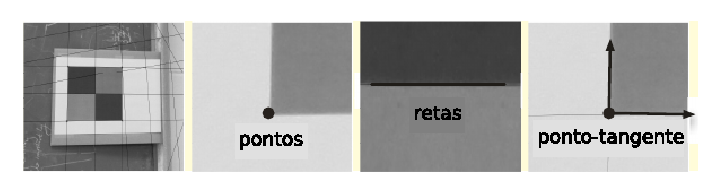
\includegraphics[width=\hsize]{astrom-objetos-geo}
\legend{Objetos utilizados para gerar equações na determinação dos parâmetros de $P$.}
\source{Kuang e \AA strom (2013).}
\label{fig.astrom-objetos-geo}
\end{figure}
\section*{Equações obtidas usando pontos.}

Dado um ponto 3D $\X$ e sua respectiva imagem em 2D $\x=(x,y,1)^\top$, a equação de projeção $\lambda\,\x=P\,\X$ nos fornece três equações. Mas, pela Subseção \ref{sec.ponto}, um ponto 2D tem apenas dois graus de liberdade apesar de suas três componentes, então dessas três equações apenas duas são linearmente independentes. Para eliminarmos o fator de escala $\lambda$ aplicamos o produto vetorial em ambos os lados da equação de projeção:
\begin{equation}\label{eq.astrom-pontos}
\begin{array}{rcl}
\lambda\,\x&=&P\,\X\\
\lambda\,[\x]_\times\x&=&[\x]_\times P\,\X\\
{\bf 0}&=&[\x]_\times P\,\X.
\end{array}
\end{equation}
\section*{Equações obtidas usando retas.} 

Uma reta 3D ${\bf L}$ pode ser representada usando um ponto $\X$ e uma direção ${\bf D}$, na forma ${\bf L}=\X+k\,{\bf D}$. Dadas a reta ${\bf L}$ e sua imagem $\lightrgb$ obtemos duas equações usando os dois pontos $\X$ e ${\bf D}$. Um ponto $\x$ pertence a uma reta $\lightrgb$ se $\lightrgb^\top\x=0$, e substituindo essa relação na equação de projeção \ref{eq.projecao} temos:
\begin{equation}\label{eq.astrom-retas}
\begin{array}{rcll}
\lightrgb^\top P\,\X&=&0&\text{se}\,\,\,k=0\\
\lightrgb^\top P(\X+k\,{\bf D})&=&0&\text{se}\,\,\,k\neq0.
\end{array}
\end{equation}  
\section*{Equações obtidas usando pontos-tangentes.}

É possível obter mais três equações se conhecemos o ponto $\X$, uma direção ${\bf D}$ através $\X$ bem como suas respectivas imagens $\x$ e ${\bf d}$. Com a correspondência $\X\leftrightarrow\x$ podemos usar a relação apresentada na Equaç\~ao \ref{eq.astrom-pontos} e conseguir duas equações. Para a terceira equação, usamos a reta definida pelos pontos na imagem, $\lightrgb=\x\times{\bf d}$, juntamente com as Equações \ref{eq.astrom-retas}, pois tomando a diferença entre tais equações e usando a reta $\lightrgb$ temos
\begin{equation}\label{eq.astrom-direcao}
\lightrgb^\top P\,{\bf D}=0.
\end{equation}  
Note que essas três equações são obtidas usando um ponto-tangente com uma direção apenas. Se usarmos ponto-tangente com mais direções, conseguimos uma equação a mais para cada direção, pois para cada ${\bf D}_i$ das $n$ direções, teremos $\lightrgb_i=\x\times{\bf d}_i$ e podemos formular as equações
\begin{equation}
[\x]_\times P\,\X={\bf 0}\quad\text{e}\quad\lightrgb_i^\top P\,{\bf D}_i=0\quad\text{para}\,\,i=1,...,n.
\end{equation}
Na tabela abaixo podemos verificar um resumo da quantidade de equações conseguidas para correspondências entre cada objeto geométrico.
\begin{center}
\begin{tabular}{|c|c|c|c|}
\hline 
{\bf ponto} & {\bf reta} & {\bf ponto com 1 tangente} & {\bf ponto com 2 tangentes} \\ 
\hline 
2 & 2 & 3 & 4 \\ 
\hline 
\end{tabular} 
\end{center}
\section*{Casos úteis.}

Com as quantidades de equações fornecidas por cada correspondência podemos formar várias combinações entre pontos, retas e ponto-tangentes para obtermos as sete equações necessárias para calcular os sete graus de liberdade de $P$. Vamos ver dois exemplos de problema mínimo.
\begin{itemize}
\item {\bf Dois pontos e um ponto-tangente (P2T1)}: com essa combinação temos três pontos e uma direção passando por um dos pontos, então podemos formar seis equações usando a Relação \ref{eq.astrom-pontos} e mais uma equação usando a Relação \ref{eq.astrom-direcao}. 

\item {\bf Um ponto-tangente com uma direção mais um ponto-tangente com duas direções (T1T2)}: temos uma reta passando por um dos pontos e duas retas passando pelo outro ponto, então podemos formar quatro equações usando \ref{eq.astrom-pontos} e mais três equações usando \ref{eq.astrom-direcao}.
\end{itemize} 

Podemos formar outros problemas mínimos conforme os apresentados aqui e vamos mostrar agora um caso supra-restringido, onde temos mais equações do que incógnitas a determinar.
\begin{itemize}
\item {\bf Quatro retas (P4L)}: Dadas quatro correspondências entre retas temos oito equações usando as Relações \ref{eq.astrom-retas}. Como precisamos de sete equações podemos usar uma delas para verificar a solução dada pelas demais.
\end{itemize}
\section*{Parametrização de $P$.}

Uma das ideias teóricas mais importantes do método e que a matriz de rotação da câmera é parametrizada com quaternions, pois desse modo produz sistemas de equações polinomiais relativamente fáceis de serem resolvidos. Utilizando quaternions, a matriz de rotação é dada por
\begin{equation*}
R=
\begin{bmatrix}
a^2+b^2-c^2-d^2&2bc-2ad&2ac+2bd\\
2ad+2bc&a^2-b^2+c^2-d^2&2cd-2ab\\
2bd-2ac&2ab+2cd&a^2-b^2-c^2+d^2
\end{bmatrix}
\end{equation*}
Se tratando de uma representação em coordenadas homogêneas podemos usar uma das variáveis para fixar a escala, assim tomando $a=1$ reduzimos o número de variáveis e facilitamos a solução do sistema de equações polinomiais.

O vetor de translação é parametrizado normalmente como ${\bf t}=(t_x,t_y,t_z)^\top$ e a matriz $[R|{\bf t}]$ se torna
\begin{equation*}
[R|{\bf t}]=
\begin{bmatrix}
a^2+b^2-c^2-d^2&2bc-2ad&2ac+2bd&t_x\\
2ad+2bc&a^2-b^2+c^2-d^2&2cd-2ab&t_y\\
2bd-2ac&2ab+2cd&a^2-b^2-c^2+d^2&t_z
\end{bmatrix}
\end{equation*}
Para completar a matriz $P$ basta aplicar, à esquerda de $[R|{\bf t}]$ a matriz de calibração $K$ conforme \ref{eq.astrom-K}.
\begin{equation*}
\begin{array}{rcl}
P&=&K\,[R|{\bf t}]\\\\
&=&
\begin{bmatrix}
1&0&0\\
0&1&0\\
0&0&w
\end{bmatrix}
\begin{bmatrix}
a^2+b^2-c^2-d^2&2bc-2ad&2ac+2bd&t_x\\
2ad+2bc&a^2-b^2+c^2-d^2&2cd-2ab&t_y\\
2bd-2ac&2ab+2cd&a^2-b^2-c^2+d^2&t_z
\end{bmatrix}\\\\
&=&
\begin{bmatrix}
a^2+b^2-c^2-d^2&2bc-2ad&2ac+2bd&t_x\\
2ad+2bc&a^2-b^2+c^2-d^2&2cd-2ab&t_y\\
w\,(2bd-2ac)&w\,(2ab+2cd)&w\,(a^2-b^2-c^2+d^2)&w\,t_z
\end{bmatrix}
\end{array}
\end{equation*} 
Substituindo $t'_z=w\,t_z$, temos que determinar as sete variáveis $\{b,c,d,t_x,t_y,t'_z,w\}$. Mas observe que as variáveis $\{t_x,t_y,t'_z\}$ são todas lineares usando as Relações \ref{eq.astrom-pontos}, \ref{eq.astrom-retas} e \ref{eq.astrom-direcao}, e portanto podem ser eliminadas do sistemas de equações restando apenas as quatro variáveis $\{b,c,d,w\}$. Depois de determinadas essas quatro variáveis, o vetor de translação pode ser recuperado por substituição. 
\section{Sistema de equações polinomiais}

Para resolver computacionalmente os sistemas de equações polinomiais decorrentes do emprego dos casos úteis na determinação de $P$, Kuang e \AA str\:om (2013) utilizam m\'etodos baseados em geometria algébrica. Primeiramente, utilizando a ferramenta {\it Macaulay2}, Grayson e Stillman (1993-2002), é verificada a existência de 20 soluções para o caso mínimo (P2T1). Para sistemas com pouca quantidade de variáveis, usar apenas o método das bases de Gr\"obner pode ser rápido e numericamente estável, mas aqui é empregado o método exposto em Byr\"od et al. (2009), que consiste basicamente em extrair a base linear a partir das bases de Gr\"obner e empregar a matriz de ação, da qual as soluções podem ser obtidas pela decomposição em autovalores. No apêndice \ref{sec.geo-algebrica} é fornecido um resumo sobre a teoria básica de geometria algébrica, bem como exemplos da utilização do método das bases de Gr\"obner e da matriz de ação para resolver sistemas computacionalmente.

\input{geo-tri-m}
\input{geo-tri-nister-m}
\input{conc-m}

% ----------------------------------------------------------
% ELEMENTOS POS-TEXTUAIS
% ----------------------------------------------------------
\backmatter
%=====================================================================
% Referencias via BibTeX
%=====================================================================
%\citeoption{abnt-options4}
%\bibliographystyle{plainnat}
%\bibliography{abnt-options4,bibliografia,exemplos}
%\bibliography{exemplos.bib}
\begin{thebibliography}{33}
\providecommand{\natexlab}[1]{#1}
\providecommand{\url}[1]{\texttt{#1}}
\expandafter\ifx\csname urlstyle\endcsname\relax
  \providecommand{\doi}[1]{doi: #1}\else
  \providecommand{\doi}{doi: \begingroup \urlstyle{rm}\Url}\fi
  
\bibitem[Ballard e Brown(1982)]{ballard-82}
BALLARD, D.~H. ; BROWN, C.~M.
\newblock \emph{Computer Vision}.
\newblock Prentice-Hall, 1982.

\bibitem[Byröd et~al.(2009)Byröd, Josephson, and Åström]{byrod}
BYR\"OD, M. ; JOSEPHSON, K. ; ÅSTR\"OM, K.
\newblock Fast and stable polynomial equation solving and its application to
  computer vision.
\newblock \emph{International Journal of Computer Vision}, 84\penalty0
  (3):\penalty0 237--255, 2009.

\bibitem[Chen(1991)]{chen}
CHEN, H.
\newblock Pose determination from line-to-plane correspondences: Existence
  condition and closed-form solutions.
\newblock \emph{IEEE Trans. Pattern Anal. Mach. Intell.}, 13\penalty0
  (6):\penalty0 530--541, 1991.

\bibitem[Cox e O'Shea(2005)]{cox-using}
LITTLE, J. ; COX, D. ; O'SHEA, D.
\newblock \emph{Using Algebraic Geometry}, volume 185 of \emph{Graduate Texts
  in Mathematics}.
\newblock Springer-Verlag, 2005.

\bibitem[Cox e O'Shea(2007)]{cox-ideals}
LITTLE, J. ; COX, D. ; O'SHEA, D.
\newblock \emph{Ideals, Varieties, and Algorithms -An Introduction to
  Computational Algebraic Geometry and Commutative Algebra}.
\newblock Undergraduate Texts in Mathematics. Springer, third edition, 2007.

\bibitem[Dhome et~al.(1989)Dhome, Richetin, Lapresté, and Rives]{dhome}
DHOME, M. ; RICHETIN, M. ; LAPRESTÉ, J. T. ; RIVES, G.
\newblock Determination of the attitude of 3d objects from a single perspective
  view.
\newblock \emph{IEEE Trans. Pattern Anal. Mach. Intell.}, 11\penalty0
  (12):\penalty0 1265--1278, 1989.

\bibitem[Fabbri e Kimia(2010{\natexlab{a}})]{fabbri-sketch}
FABBRI, R. ; KIMIA, B.~B.
\newblock {3D} curve sketch: Flexible curve- based stereo reconstruction and
  calibration.
\newblock \emph{CVPR}, 2010{\natexlab{a}}.

\bibitem[Fabbri e Kimia(2011)]{tese-fabbri}
FABBRI, R. ; KIMIA, B.~B.
\newblock \emph{Multiview Differential Geometry in Application to Computer
  Vision}.
\newblock PhD thesis, Brown University, may 2011.

\bibitem[Fabbri e Kimia(2015)]{fabbri-drawing}
FABBRI, R. ; KIMIA, B.~B.
\newblock From multiview image curves to {3D} drawings.
\newblock \emph{CVPR}, 2015.

\bibitem[Fabbri e Kimia(2010{\natexlab{b}})]{Fabbri:Kimia:CVPR10}
FABBRI, R. ; KIMIA, B.~B.
\newblock {3D} curve sketch: Flexible curve-based stereo reconstruction and
  calibration.
\newblock In \emph{Proceedings of the IEEE Conference on Computer Vision and
  Pattern Recognition}, San Francisco, California, USA, 2010{\natexlab{b}}.
  IEEE Computer Society Press.

\bibitem[Fabbri et~al.(2012)Fabbri, Giblin, and
  Kimia]{Fabbri:Giblin:Kimia:ECCV12}
FABBRI, R. ; GIBLIN, P. J. ; KIMIA, B. B.
\newblock Camera pose estimation using first-order curve differential geometry.
\newblock In \emph{Proceedings of the IEEE European Conference in Computer
  Vision}, Lecture Notes in Computer Science. Springer, 2012.

\bibitem[Faugeras(1993)]{faugeras93three}FAUGERAS, O.
\newblock \emph{Three-dimensional computer vision: a geometric viewpoint}.
\newblock MIT press, 1993.

\bibitem[Faugeras et~al.(2001)Faugeras, Luong, and Papadopoulo]{Faugeras}
FAUGERAS, O. ; LUONG, Q. T. ; PAPADOPOULO, T.
\newblock \emph{The geometry of multiple images - the laws that govern the
  formation of multiple images of a scene and some of their applications,}.
\newblock MIT Press, 2001.

\bibitem[Fischler e Bolles(1981)]{fischler}
FISCHLER, M. ; BOLLES, R.
\newblock Random sample consensus: A paradigm for model fitting with
  applications to image analysis and automated cartography.
\newblock \emph{Communications of the ACM}, 24\penalty0 (6):\penalty0 381--395,
  1981.

\bibitem[Forsyth e Ponce(2003)]{forsyth}
FORSYTH, D.~A. ; ~PONCE, J.
\newblock \emph{Computer Vision, A Modern Approach}.
\newblock Prentice Hall, 2003.

\bibitem[Grayson e Stillman(1993-2002)]{macaulay2}
GRAYSON, D. ; ~STILLMAN, M.
\newblock Macaulay 2, an open source computer algebra software., 1993-2002.
\newblock URL \url{www.math.uiuc.edu/Macaulay2/}.

\bibitem[Hartley e Zisserman(2004)]{Hartley2004}
HARTLEY, R.~I. ; ZISSERMAN, A.
\newblock \emph{Multiple View Geometry in Computer Vision}.
\newblock Cambridge University Press, ISBN: 0521540518, second edition, 2004.

\bibitem[Hartley e Li(2012)]{HartleyLi}
HARTLEY, R.~I. ; Li, H.
\newblock An efficient hidden variable approach to minimal-case camera motion
  estimation.
\newblock \emph{IEEE Transactions on Pattern Analysis and Machine Intelligence
  (PAMI)}, 34\penalty0 (23):\penalty0 2303--2314, dezembro 2012.

\bibitem[Kuang e {\AA}str{\"o}m(2013)]{bib:kuang}
KUANG, Y. ; {\AA}STR{\"O}M, K.
\newblock Pose estimation with unknown focal length using points, directions
  and lines.
\newblock In \emph{Proceedings of IEEE International Conference on Computer
  Vision (ICCV2013)}, pages 529--536, 2013.

\bibitem[Kukelova et~al.(2008{\natexlab{a}})Kukelova, Bujnak, and
  Pajdla]{kukelova}
KUKELOVA, Z. ; BUJNAK, M. ; PAJDLA, T.
\newblock Automatic generator of minimal problem solvers.
\newblock In \emph{ECCV (3)}, pages 302--315, 2008{\natexlab{a}}.

\bibitem[Kukelova et~al.(2008{\natexlab{b}})Kukelova, Bujnak, and
  Pajdla]{pajdla}
KUKELOVA, Z. ; BUJNAK, M. ; PAJDLA, T.
\newblock Polynomial eigenvalue solutions to the 5-pt and 6-pt relative pose
  problems.
\newblock In \emph{BMVC}, 2008{\natexlab{b}}.

\bibitem[Köser e Koch(2008)]{koser}
K\"OSER, K. ; KOCH, R.
\newblock Differential spatial resection - pose estimation using a single local
  image feature.
\newblock In David~A. Forsyth, Philip H.~S. Torr, and Andrew Zisserman,
  editors, \emph{ECCV (4)}, pages 312--325, 2008.

\bibitem[Longuet-Higgins(1981)]{Longuet}
LONGUET-HIGGINS, H.~C.
\newblock A computer algorithm for reconstructing a scene from two projections.
\newblock \emph{Nature}, 293:\penalty0 133--135, Setembro 1981.

\bibitem[Luong e Viéville(1996)]{luong}
LUONG, Q.~T. ; VIÉVILLE, T.
\newblock Canonical representations for the geometries of multiple pro- jective
  views.
\newblock \emph{Computer Vision and Image Understanding}, pages 193--229,
  setembro 1996.

\bibitem[Matthies et~al.(2007)Matthies, Maimone, Johnson, Cheng, Willson,
  Villalpando, Goldberg, Huertas, Stein, and Angelova]{mars-rover}
MATTHIES, L. et~al. 
%; MAIMONE, M. ; JOHNSON, A. ; CHENG, Y. ; WILLSON, R. ; Villalpando, C.
%; GOLDBERG, S. ; HUERTAS, A. ; STEIN, A. ; ANGELOVA, A.
\newblock Computer vision on mars.
\newblock \emph{International Journal of Computer Vision}, 2007.

\bibitem[Nistér e Schaffalitzky(2006)]{2503343}
NISTÉR, D. ; SCHAFFALITZKY, F.
\newblock {Four Points in Two or Three Calibrated Views: Theory and Practice}.
\newblock \emph{International Journal of Computer Vision}, 67:\penalty0
  211--231, 2006.

\bibitem[Faugeras e Maybank(1992)]{faugeras92}
LUONG, Q. ; FAUGERAS, O.~D. ; MAYBANK, S.
\newblock Camera self-calibration: Theory and experiments.
\newblock In \emph{European Conference on Computer Vision}, volume LNCS 588,
  page 321–334. Springer-Verlag, 1992.

\bibitem[N{\"o}lle et~al. (1994)]{haralick}
N{\"O}LLE, M. et~al.
\newblock Review and analysis of solutions of the three point perspective pose
  estimation problem.
\newblock In \emph{Int. J. of Computer Vision.}, page 331–356, 1994.

\bibitem[Ramalingam et~al.(2011)Ramalingam, Bouaziz, and Sturm]{ramalingam}
RAMALINGAM, S. ; BOUAZIZ, S. ; STURM, P.~F.
\newblock Pose estimation using both points and lines for geo-localization.
\newblock In \emph{ICRA}, pages 4716--4723. IEEE, 2011.

\bibitem[Schmid e Zisserman(2000)]{Schmid00}
SCHMID, C. ; ZISSERMAN, A.
\newblock The geometry and matching of lines and curves over multiple views.
\newblock \emph{International Journal of Computer Vision}, 40\penalty0
  (3):\penalty0 199--233, 2000.

\bibitem[Semple e Kneebone(1952)]{kneebone}
SEMPLE, J.~G. ; KNEEBONE, G.~T.
\newblock \emph{Algebraic Projective Geometry}.
\newblock Oxford University Press, 1952.

\bibitem[Spetsakis e Aloimonos(1990)]{original-trifocal-retas}
SPETSAKIS, M.~E. ; ALOIMONOS, J.
\newblock Structure from motion using line correspondences.
\newblock \emph{The International Journal of Computer Vision}, 1990.

\bibitem[Springer(1964)]{springer64}
SPRINGER, C.~E.
\newblock \emph{Geometry and Analysis in Projective Space.}
\newblock Freeman, 1964.  
\end{thebibliography}
%=====================================================================

%=====================================================================
%\postextualchapter*{Glossário}
%=====================================================================
%\definicao{termo 1}{significado}
%\definicao{termo 2}{significado}
%\definicao{termo 3}{significado}
% ----------------------------------------------------------
% Apêndices (opcionais)
% ----------------------------------------------------------
% ---
% Inicia os apêndices
% ---
\appendix
%=====================================================================
\postextualchapter{Alguns conceitos e definições de álgebra linear}\label{sec.Apen-A}
%=====================================================================

Esta seção do apêndice se destina a apresentar algumas ferramentas da álgebra linear necessárias ao entendimento de algumas seções da dissertação, funcionando como complementação dessas seções.

\section{A matriz anti-simétrica $[{\bf v}]_\times$}
Dado um vetor ${\bf v}=(v_1,v_2,v_3)^\top$, é possível construir uma matriz anti-simétrica com as componentes de ${\bf v}$ na forma
\begin{equation*}
[{\bf v}]_\times=
\begin{bmatrix}
0&-v_3&v_2\\
v_3&0&-v_1\\
-v_2&v_1&0
\end{bmatrix},
\end{equation*}
onde a notação $[{\bf v}]_\times$ indica uma relação com o produto vetorial entre um vetor qualquer ${\bf u}$ e ${\bf v}$. 
\begin{equation*}
{\bf v} \times {\bf u} = [{\bf v}]_\times {\bf u} = ({\bf v}^\top [{\bf u}]_\times)^\top
\end{equation*}
Sabemos que o produto vetorial entre um vetor e ele mesmo é sempre o vetor nulo, portanto o vetor ${\bf v}$ é o vetor nulo à direita e à esquerda de $[{\bf v}]_\times$. Desta forma, esta matriz anti-simétrica será sempre definida por seu vetor nulo.  

Observe, ainda, que uma matriz anti-simétrica qualquer $M$ satisfaz a relação ${\bf v}^\top M\,{\bf v}=0.$ Pois,
\begin{equation*}
\begin{array}{rcl}
{\bf v}^\top M\,{\bf v}
&=&
\begin{pmatrix}
v_1&v_2&v_3
\end{pmatrix}
\begin{bmatrix}
0&m_{12}&m_{13}\\
-m_{12}&0&m_{23}\\
-m_{13}&-m_{23}&0
\end{bmatrix}
\begin{pmatrix}
v_1\\
v_2\\
v_3
\end{pmatrix}\\
&=&
\begin{pmatrix}
-v_2 m_{12}-v_3 m_{13}&v_1 m_{12}-v_3 m_{23}&v_1 m_{13}+v_2 m_{23}
\end{pmatrix}
\begin{pmatrix}
v_1\\
v_2\\
v_3
\end{pmatrix}\\
&=&
-v_1 v_2 m_{12}-v_1 v_3 m_{13}+v_1 v_2 m_{12}-v_2 v_3 m_{23}+v_1 v_3 m_{13}+v_2 v_3 m_{23}\\
&=&0.
\end{array}
\end{equation*}

%\subsection*{O método das potências para autovalores}
%Segundo \citep{cox-using}, o método das potências é baseado no fato de que uma matriz $A$ possui um único autovalor dominante, ou seja, um autovalor $\lambda$ que satisfaz $\begin{Vmatrix}\lambda\end{Vmatrix} > \begin{Vmatrix}\mu\end{Vmatrix}$ para todos os outros autovalores $\mu$ de $A$. Basta aplicar uma alteração no método caso a matriz não tenha um autovalor dominante. O método é iterativo e consiste em estipular uma estimativa inicial para o autovetor ${\bf v}_k$ e determinar o autovetor ${\bf v}_{k+1}$ em cada iteração fazendo
%
%\begin{equation*}
%{\bf v}_{k+1}=A\,{\bf v}_k,
%\end{equation*}
%onde aproximamos um autovetor relativo a $\lambda$ quando $k\rightarrow \infty$. Encontrada a aproximação para o autovetor podemos determinar o autovalor dominante correspondente aplicando o \textit{quociente de Rayleigh}, pois sendo ${\bf v}$ o autovetor relativo a $\lambda$ temos
%
%\begin{equation*}
%A\,{\bf v}=\lambda\,{\bf v},
%\end{equation*}
%e aplicando o produto escalar na equação
%
%\begin{equation*}
%\begin{array}{rcl}
%A\,{\bf v}&=&\lambda\,{\bf v}\\
%(A\,{\bf v})\cdot{\bf v}&=&\lambda\,({\bf v}\cdot{\bf v})\\
%\lambda&=&\frac{(A\,{\bf v})\cdot{\bf v}}{{\bf v}\cdot{\bf v}}.
%\end{array}
%\end{equation*}
%
%Para evitar problemas de overflow/underflow podemos alterar a escala do vetor, calculando a norma do vetor ou dividindo o vetor pela maior de suas componentes em cada iteração. Sempre que dividirmos o vetor pela maior de suas componentes todas as componentes vão se manter entre $-1$ e $1$. Optando pela norma basta computar $\begin{Vmatrix}A\,{\bf v}_k\end{Vmatrix}$ a cada iteração. 
%
%
%Se a matriz não possui um único autovalor dominante o método pode não convergir, ou podemos precisar determinar os demais autovalores. Nesses casos, devemos fazer uma modificação na matriz de forma a garantir a convergência. O procedimento consiste em calcular o autovalor mais próximo de um $s$ arbitrário, de uma matriz
%
%\begin{equation*}
%A'=(A-s\,I)^{-1}
%\end{equation*}
%onde para quase todas as escolhas de $s$ a matriz $A'$ terá um único autovalor dominante. Sendo $\lambda'$ o autovalor dominante de $A'$, o autovalor dominante de $A$ é dado por
%
%\begin{equation*}
%\lambda=\frac{1}{\lambda'}+s
%\end{equation*} 
%onde $\lambda$ será o autovalor mais próximo de $s$. Este procedimento permite procurar por todos os autovalores de uma matriz, dada uma boa estimativa para $s$, como se desejaria fazer utilizando o método de Newton-Raphson para o polinômio característico, o qual não é muito utilizado na prática.

\section{A decomposição SVD}
Uma das formas de se obter a decomposição em valores singulares de uma matriz $A$ é aplicando a decomposição em autovalores na matriz  $A^\top A$. Assim, queremos determinar a decomposição
\begin{equation*}
A=U\,D\,V^\top
\end{equation*} 
onde as matrizes $U$ e $V$ são ortogonais. Observe que calculando $A^\top A$ temos
\begin{equation*}
\begin{array}{rcl}
A^\top A&=&V\,D\,U^\top U\,D\,V^\top\\
&=&V\,D^2 V^{-1},
\end{array}
\end{equation*}
onde $V\,D^2 V^{-1}$ é uma decomposição em autovalores.

Desta forma, aplicando a decomposição em autovalores na matriz $A^\top A$, conseguimos diretamente a matriz $V^\top$ da decomposição SVD, e basta extrair a raiz quadrada das componentes da diagonal de $D$ para obtermos os valores singulares. Com uma inversão de matrizes podemos obter a matriz $U$:
\begin{equation*}
\begin{array}{rcll}
A&=&U\,D\,V^\top &\Rightarrow\\
U&=&A\,(D\,V^\top)^{-1} &\Rightarrow\\
U&=&A\,V^{-\top}D^{-1}.
\end{array}
\end{equation*}
Não são todos os problemas que envolvem a decomposição SVD que necessitam que sejam calculadas todas a matrizes. Existem problemas onde não é necessário o cálculo da matriz $U$ por exemplo. Então a complexidade computacional vai depender também daquilo que é necessário ao problema.

\section{A pseudo-inversa de $P$}
Primeiramente precisamos definir a inversa de uma matriz quadrada diagonal. Sendo $D$ essa matriz, sua inversa será
\begin{empheq}{align*}
D_{ii}^+=
\empheqlbrace{
\begin{array}{c}
0\,\,\,, \,\,\text{se}\,\,\,D_{ii}=0\\
\frac{1}{D_{ii}}\,\,,\,\,\,\text{se}\,\,\,D_{ii}\neq0.
\end{array}}
\end{empheq}
A matriz $P_{3\times4}$ tem menor quantidade de linhas do que colunas, e nesse caso devemos extender a matriz $P$ acrescentando uma linha de zeros para que a mesma se torne uma matriz quadrada. Não poderemos inverter tal matriz quadrada pois com uma linha de zeros ela será singular. Assim, aplicamos a decomposição SVD e em seguida definimos a pseudo-inversa. Se
\begin{equation*}
P=U\,D\,V^\top
\end{equation*}
é a decomposição SVD, podemos definir a pseudo-inversa como
\begin{equation*}
P^+=V\,D^+U^\top.
\end{equation*}
De fato, podemos verificar essa definição usando $D^+$ e o fato de que as matrizes $U$ e $V$ são ortogonais (suas inversas são suas transpostas).
\begin{equation*}
\begin{array}{rcl}
P^+P&=&V\,D^+U^\top\,U\,D\,V^\top\\
&=&V\,D^+I\,D\,V^\top\\
&=&V\,D^+D\,V^\top\\
&=&V\,I\,V^\top\\
&=&V\,V^\top\\
&=&I
\end{array}
\end{equation*}
Uma das maneiras de realizar a decomposição SVD é aplicando a decomposição em autovalores, a qual fornece a matriz $V$ e fornece quase diretamente os valores singulares. Em seguida, fica relativamente fácil obter a matriz $U$.

%=====================================================================
\postextualchapter{Alguns conceitos e definições de geometria algébrica}\label{sec.geo-algebrica}
%=====================================================================


Esta seção se destina a apresentar um resumo das definições básicas em Geometria Algébrica, bem como alguns conceitos e definições mais avançados necessários ao entendimento do procedimento de solução de sistemas de equações polinomiais. Para acessar um detalhamento maior da teoria juntamente com as demonstrações dos teoremas, o leitor pode consultar os livros Cox et al. (2005) e Cox et al. (2007).

\section{Definições básicas}

A Geometria Algébrica tem como objetivo principal de estudos as variedades algébricas, os objetos geométricos
formados pelos pontos que são soluções de um sistema de equações polinomiais. Para realizar esse estudo, utiliza técnicas de álgebra comutativa em conjunto com a linguagem geométrica.

{\it Monômios} são o produto de $n$ variáveis da forma $x_1^{\alpha_1}\cdot x_2^{\alpha_2} \cdot ... \cdot x_n^{\alpha_n}$ onde os expoentes são números inteiros não-negativos. O grau total de um monômio é a soma dos expoentes das variáveis e é denotado por $|\alpha|=\alpha_1+\alpha_2+...+\alpha_n$, e para simplificar a notação é adotada a convenção onde $\alpha=(\alpha_1,\alpha_2,...,\alpha_n)$ é o vetor dos expoentes e $x^\alpha=x_1^{\alpha_1}\cdot x_2^{\alpha_2} \cdot ... \cdot x_n^{\alpha_n}$ é a representação do monômio.

{\it Polinômios} são combinações lineares dos monômios denotados por
\begin{equation*}
f=\sum_\alpha a_\alpha x^\alpha,\quad\text{onde}\quad a_\alpha\in k.
\end{equation*} 
Os coeficientes desses polinômios pertencem a um conjunto numérico denominado {\it corpo}, denotado por $k$, que pode ser o conjunto dos números complexos ou reais, por exemplo. Informalmente, corpo é um conjunto fechado para adição, subtração, multiplicação e divisão com suas propriedades usuais. O conjunto de todos os polinômios nas $n$ variáveis definidas num corpo $k$ é denotado por $k[x_1,...,x_n]$.

Se estivermos trabalhando com pouca variáveis podemos utilizar $x$, $y$ e $z$ e como exemplo temos
\begin{equation*}
f=2x^3y^2z+\frac{2}{3}y^3z^3-3xyz+y^2\quad\in\quad\mathbb{Q}[x,y,z],
\end{equation*} 
onde
\begin{itemize}
\item os {\it coeficientes} são 2, $\frac{2}{3}$, -3 e 1,
\item os {\it termos} são cada monômio junto com o respectivo coeficiente
\item o {\it grau total} do polinômio é o grau do monômio de maior grau; no caso temos dois monômios com grau 6.
\end{itemize}

A soma e o produto de dois polinômios também são polinômios, mas um polinômio $f$ divide um polinômio $g$ apenas se existe um polinômio $h$ onde $g=f\,h$. Assim, entre polinômios ficam satisfeitos os axiomas de adição e multiplicação em um corpo, mas não a existência de um inverso multiplicativo, pois por exemplo, $f=\frac{1}{x}$ não é um polinômio. Os elementos que obedecem essa estrutura formam um {\it anel comutativo}, com estudos feitos com base na {\it álgebra comutativa}, e por isso o conjunto $k[x_1,...,x_n]$ é chamado {\it anel de polinômios}.

\section{Ideal e variedade}
Um espaço $n$-dimensional num corpo $k$ é definido como
\begin{equation*}
k^n=\{(a_1,...,a_n)\,/\, a_1,...,a_n\in k\},
\end{equation*}
e é possível relacionar polinômios com um espaço $n$-dimensional observando que um polinômio nos dá uma função
\begin{equation*}
f:k^n\rightarrow k\quad\text{com}\quad f=\sum_\alpha a_\alpha x^\alpha\quad \in\quad k[x_1,...,x_n].
\end{equation*}
A capacidade em tratar polinômios como funções é o que possibilita ligar álgebra e geometria através das chamadas {\it variedades}, definida a seguir e denotada por ${\bf V}$.
\begin{equation*}
{\bf V}(f_1,...,f_s)=\{(a_1,...,a_n)\in k^n/\, f_i(a_1,...,a_n)=0, \,\forall\,\, 1\le i\le s\}.
\end{equation*}
Portanto, variedades podem ser entendidas como o conjunto de vetores que são solução de um sistema de equações polinomiais, e que fornecem uma representação geométrica para a solução do sistema sempre que possível.

Como exemplo, temos na Figura \ref{fig.variedades} a representação geométrica das variedades ${\bf V}(xy-x^3+1)$ e ${\bf V}(-x^2-y+z)$, onde cada ponto no plano e no espaço é representado pelas soluções de $xy-x^3+1=0$ e $-x^2-y+z=0$, respectivamente.
\begin{figure}[!htb]{\textwidth}
\caption{Variedades.}
\subfloat[]{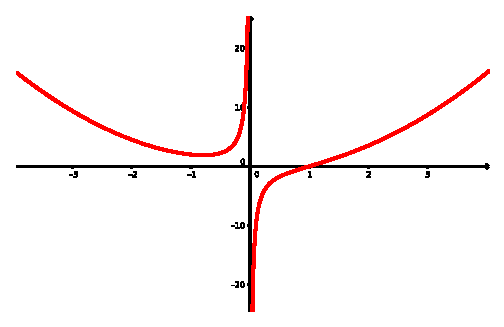
\includegraphics[width=.57\hsize]{variedade-1}}\hfill
\subfloat[]{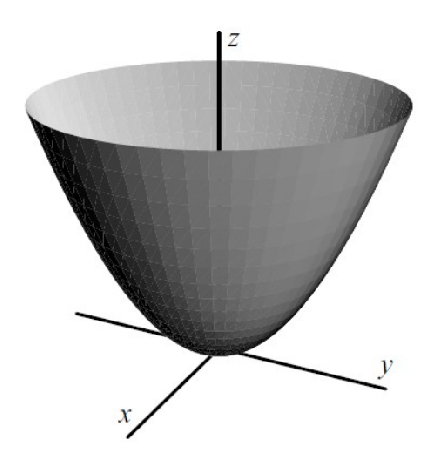
\includegraphics[width=.4\hsize]{variedade-3D}}\hfill
\legend{As representações geométricas podem ser obtidas usando as funções ({\tt a}) $y=\frac{x^3-1}{x}$ e ({\tt b}) $z=x^2+y$.}
\source{({\tt a}) O autor. ({\tt b}) Cox et al. (2005).}
\label{fig.variedades}
\end{figure} 

{\it Ideal} é um subconjunto de $k[x_1,...,x_n]$ denotado por $I$ que satisfaz as condições:
\begin{itemize}
\item $0\in I$;
\item $f,g\,\in I \Rightarrow (f+g)\in I$;
\item $f \in I$ e $h \in k[x_1,...,x_n] \Rightarrow h\,f \in I$. 
\end{itemize}

Se $f_1,...,f_s$ são polinômios em $k[x_1,...,x_n]$ então podemos definir um ideal através desses polinômios que são chamados de {\it base} do ideal, usando a notação
\begin{equation*}
I=\left\langle f_1,...,f_s \right\rangle = \{\sum_{i=1}^s h_if_i\,:\,h_1,...,h_s \in k[x_1,...,x_n]\}.
\end{equation*}
Por exemplo, para sabermos se o polinômio $x^2-2x+2-y$ pertence ao ideal $\left\langle x-1-t\,,\,y-1-t^2 \right\rangle$ devemos verificar se é possível escrevê-lo como combinação das bases desse ideal, 
\begin{equation*}
x^2-2x+2-y=(x-1+t)(x-1-t)+(-1)(y-1-t^2).
\end{equation*}
Um mesmo ideal pode ser formado por bases diferentes e, quando isso acontece, as variedades definidas por cada base também são iguais, ou seja
\begin{equation*}
\left\langle f_1,...,f_s \right\rangle = \left\langle g_1,...,g_s \right\rangle \Rightarrow {\bf V}(f_1,...,f_s)={\bf V}(g_1,...,g_s).
\end{equation*}
Por exemplo, temos a seguir um ideal formado por bases diferentes (podemos verificar que se trata do mesmo ideal escrevendo os polinômios da esquerda como combinação dos polinômios da direita e reciprocamente) e que possuem variedades iguais:
\begin{equation*}
\left\langle 2x^2+3y^2-11\,,\,x^2-y^2-3 \right\rangle = \left\langle x^2-4\,,\,y^2-1 \right\rangle,\,\, \text{logo}
\end{equation*}
\begin{equation}\label{eq.variedades}
{\bf V}(2x^2+3y^2-11\,,\,x^2-y^2-3)={\bf V}(x^2-4\,,\,y^2-1)=\{(\pm2,\pm1)\}.
\end{equation}
Observe que todos os polinômios de um ideal terão o mesmo conjunto variedade gerado pelos polinômios da base. Observe ainda, que a base de um ideal pode ser pensada como um sistema de equações polinomiais, e que para encontrarmos o conjunto solução do sistema (variedade) podemos converter a base dada numa base mais simples conforme a relação \ref{eq.variedades}. Mais à frente veremos que é exatamente esse o procedimento realizado pelas bases de Gr\"obner.

\section{As bases de Gr\"obner}

Para sabermos se um polinômio $f$ pertence a um ideal devemos dividir $f$ pelas bases do ideal e verificar se o resto é zero, pois assim $f$ pode ser escrito como combinação dos polinômios da base. Na divisão de polinômios de uma variável o resto é único, mas para polinômios de mais de uma variável, tanto o resto como os quocientes podem variar dependendo da ordem dos divisores e da ordenação de monômios escolhida ({\it lexicográfica, lexicográfica graduada e lexicográfica graduada reversa}). Para detalhes sobre divisão de polinômios de várias variáveis consultar Cox et al. (2005). 

Por exemplo, vamos verificar se o polinômio $f=xy^2-x$ pertence ao ideal $I=\left\langle xy+1\,,\,y^2-1 \right\rangle$. Efetuando a divisão de $f$ por $\{xy+1\,,\,y^2-1\}$ nesta ordem, obtemos
\begin{equation*}
xy^2-x=y(xy+1)+0(y^2-1)+(-x-y)
\end{equation*}  
com resto $-x-y$. Mas efetuando a divisão na ordem $\{y^2-1\,,\,xy+1\}$ teremos
\begin{equation*}
xy^2-x=x(y^2-1)+0(xy+1)+0
\end{equation*} 
com resto zero. Assim, $f\in I$ e vemos que, dada uma base qualquer de $I$, o resto zero é uma condição suficiente para que $f\in I$ mas não é uma condição necessária. 

Precisamos de uma base que facilite verificar se um polinômio pertence a um ideal, e as bases de Gr\"obner tem essa propriedade, pois um polinômio $f$ quando dividido pelas bases de Gr\"obner deixa resto único, não importanto a ordem dos divisores (base do ideal). Assim, sendo $G=\{g_1,...,g_t\}$ uma base de Gr\"obner, então 
\begin{equation*}
f\in I \Leftrightarrow \text{o resto da divisão de $f$ por $G$ é zero}.
\end{equation*}
Essa propriedade é tão importante que às vezes é tomada como a própria definição para as bases de Gr\"obner. O resto da divisão de um polinômio $f$ por $G=\{g_1,...,g_t\}$ é denotado por $\overline{f}^G$. Por exemplo, dividindo $f=x^5y$ por $G=\{x^2y-y^2\,,\,x^4y^2-y^2\}$ é $\overline{x^5y}^G=xy^3$, pois
\begin{equation*}
x^5y=(x^3+xy)(x^2y-y^2)+(0)(x^4y^2-y^2)+xy^3.
\end{equation*}
Para verificarmos se uma base é uma base de Gr\"obner utilizamos o {\it critério de Buchberger}, e caso não seja, toda base de um ideal pode ser convertida numa base de Gr\"obner utilizando o {\it algoritmo de Buchberger}. 

\section{Resolvendo sistemas com as bases de Gr\"obner}

Considere o sistema
\begin{empheq}[left=\empheqlbrace]{align*}
x^2+y^2+z^2&=1\\
x^2+z^2-y&=0\\
x-z&=0,
\end{empheq}
cujas soluções podem ser obtidas como a extração do conjunto variedade do ideal
\begin{equation*}
I=\left\langle x^2+y^2+z^2-1\,,\,x^2+z^2-y\,,\,x-z\right\rangle. 
\end{equation*}
Como toda base de um ideal pode ser convertida numa base de Gr\"obner, aplicando o algoritmo de Buchberger calculamos uma nova base para o ideal
\begin{equation*}
I=\left\langle x-z\,,\,-y+2z^2\,,\,z^4+\frac{1}{2}z^2-\frac{1}{4}\right\rangle. 
\end{equation*}
Como um ideal com bases diferentes possui o mesmo conjunto variedade, podemos converter as bases de Gr\"obner num novo sistema que terá o mesmo conjunto solução do anterior,
\begin{empheq}[left=\empheqlbrace]{align*}
x-z&=0\\
-y+2z^2&=0\\
z^4+\frac{1}{2}z^2&=\frac{1}{4}.
\end{empheq}
Note que a última equação do sistema depende apenas de uma variável, que pode ser obtida através de um método numérico. O {\it teorema da eliminação} garante que, definida uma ordenação de monômios, as variáveis de um sistema são eliminadas de acordo com a precedência dessa ordem. Depois de calculada a primeira variável, por retro-substituição podemos determinar o valor das variáveis restantes, onde tal retro-substituição é garantida, sob determinadas condições, pelo {\it teorema da extensão}. Alguns softwares de computação algébrica (como Maple) possuem pacotes para computação das bases de Gr\"obner. O procedimento apresentado aqui para solução de sistemas possui algumas deficiências que serão comparadas com o procedimento a seguir no final do apêndice.

\section{Álgebra de um espaço dimensional finito}

Na divisão de um polinômio $f\in k[x_1,...,x_n]$ por uma base de Gr\"obner $G$ obtemos a expansão
\begin{equation*}
f=h_1g_1+...+h_tg_t+\overline{f}^G,
\end{equation*} 
onde $\overline{f}^G$ é uma combinação de monômios que não são divisíveis pelos termos líderes dos polinômios de $G$. Mas existem outros polinômios em $k[x_1,...,x_n]$ que deixam o mesmo resto que $f$ na divisão por $G$. Assim $f$ definde uma {\it classe de equivalência} dada por
\begin{equation*}
[f]=\{p\in k[x_1,...,x_n]\,/\,p\equiv f\, \text{mod}\, I\}.
\end{equation*}
Ou seja, assim como temos os polinômios que pertencem ao ideal $I$, temos também o conjunto dos polinômios que não pertencem ao ideal, e cada um desses polinômios pertence à sua classe de equivalência. O conjunto de todas as classes de equivalência de um ideal forma um anel denominado {\it anel quociente}, denotado por
\begin{equation*}
k[x_1,...,x_n]/I=\{[f]\,/\,f\in k[x_1,...,x_n]\}.
\end{equation*}

Quando multiplicamos dois restos de um ideal, $\overline{f}^G\cdot\overline{p}^G$, podemos obter um polinômio que pertence ao ideal, mas quando somamos dois restos ou multiplicamos um resto por um escalar, o polinômio gerado continua pertencendo ao anel quociente $k[x_1,...,x_n]/I$. Por essa e outras características, temos que esse anel tem a estrutura de um {\it espaço vetorial} e é denominado {\it Álgebra}. Os monômios que não são divisíveis pelos termos líderes de $G$ formam uma base para essa Álgebra, denominada {\it base linear}. Considere como exemplo o ideal gerado por 
\begin{equation}\label{eq.base-G}
G=\{x^2+\frac{3xy}{2}+\frac{y^2}{2}-\frac{3x}{2}-\frac{3y}{2}\,,\,xy^2-x\,,\,y^3-y\},
\end{equation}
cujo polinômios têm os termos líderes dados por $\{x^2\,,\,xy^2\,,\,y^3\}$. Extraindo os monômios que não são divisíveis pelos termos líderes formamos a base linear
\begin{equation*}
B=\{1\,,\,x\,,\,y\,,\,xy\,,\,y^2\},
\end{equation*}
onde os cinco monômios são uma base do espaço vetorial para a álgebra $A={\mathbb C}[x,y]/I$. Assim, todo polinômio que não pertence a $I$ pode ser escrito como uma {\it combinação linear} dos monômios de $B$.

A base linear $B$ tem dimensão finita e sempre terá desde que sejam satisfeitas as condições do {\it teorema da finitude}, para o qual a principal condição é que sendo $G$ uma base de Gr\"obner para um ideal $I \subset k[x_1,...,x_n]$, então para cada $1\le i\le n$, existe um $m_i\ge 0$ tal que $x_i^{m_i}$ é o termo líder de algum $g\in G$. Ou seja, considerando a base $G$ na relação \ref{eq.base-G}, se por exemplo $y^{m_y}$ não pertencesse ao conjunto dos termos líderes para algum $m_y$, não teríamos um expoente que pudesse restringir $y$ a pertencer à base $B$, e esta seria infinita.

\section{Resolvendo sistemas com autovalores e autovetores}

A ideia principal é explorar a estrutura de $A=k[x_1,...,x_n]/I$ para estimar o valor de alguma funcão $f$ nos valores de $V$. Observe que nossa tarefa é encontrar os valores de $x_i\in (x_1,...,x_n)$ onde $(x_1,...,x_n)\in V$, assim podemos tomar a função $f=x_i$, pois estimar o valor para $f$ cumprirá a tarefa de encontrar os valores de cada componente do vetor solução.

Para determinar o valor de cada variável é definido um operador linear $m_{x_i}$ como a multiplicação de cada variável $x_i$ pelos polinômios $b$ da base $B$.
\begin{equation*}
m_{x_i}:A\rightarrow A\quad\text{onde}\quad m_{x_i}([b])=x_i\cdot[b].
\end{equation*} 
Desta forma, os possíveis valores para a variável $x_i$ são computados através da decomposição em autovalores da matriz $m_{x_i}$. Por definição em Álgebra Linear, para encontrarmos a matriz $m_{x_i}$,  devemos expandir $p_j=x_i\cdot b_j$ em termos da base $B$, e tomar a transposta da matriz dos coeficientes dessa expansão.

Contudo, multiplicando dois elementos de $A$, não podemos garantir que o resultado $p_j$ seja um elemento de $A$ que possa ser escrito como combinação linear dos elementos de $B$. Assim, devemos escrever a expansão de $p_j$ em termos dos elementos da base $G$ para obter o resto $\overline{p}^{G}$. Como todo polinômio
\begin{equation}\label{eq.resto-mod}
p\equiv\overline{p}^{G}\,\text{mod}\,I,
\end{equation} 
podemos expandir $\overline{p}^{G}$ ao invés de $p$. 

Como exemplo, vamos calcular as soluções do sistema formado pelos polinômios da base $G$ em \ref{eq.base-G},
\begin{empheq}[left=\empheqlbrace]{align*}
x^2+\frac{3xy}{2}+\frac{y^2}{2}-\frac{3x}{2}-\frac{3y}{2}&=0\\
xy^2-x&=0\\
y^3-y&=0,
\end{empheq}
com termos lideres $\{x^2\,,\,xy^2\,,\,y^3\}$ e base $B=\{1\,,\,x\,,\,y\,,\,xy\,,\,y^2\}$. Determinando primeiramente os valores para $x$ temos que $m_x(b_j)=x\cdot b_j$, portanto
\begin{equation*}
\begin{array}{rcccl}
x\cdot1 &= &x& = &0 \cdot 1 + 1 \cdot x + 0 \cdot y + 0 \cdot xy + 0 \cdot y^2\\\\
x \cdot x &= &x^2&=& 0 \cdot 1 + \frac{3}{2} \cdot x + \frac{3}{2} \cdot y - \frac{3}{2} \cdot xy\, – \,\frac{1}{2} \cdot y^2\\\\
x \cdot y &=& xy &= &0 \cdot 1 + 0 \cdot x + 0 \cdot y + 1 \cdot xy + 0 \cdot y^2\\\\
x \cdot xy &=& x^2y &= &0 \cdot 1\, – \,\frac{3}{2} \cdot x \,–\, \frac{1}{2} \cdot y + \frac{3}{2} \cdot xy + \frac{3}{2} \cdot y^2\\\\
x \cdot y^2 &= &xy^2& =& 0 \cdot 1 + 1 \cdot x + 0 \cdot y + 0 \cdot xy + 0 \cdot y^2.
\end{array}
\end{equation*}
Tomando a transposta dos coeficientes temos a denominada {\it matriz de ação},
\begin{equation*}
m_x=
\begin{bmatrix}
0&0&0&0&0\\\\
1&\frac{3}{2}&0&-\frac{3}{2}&1\\\\
0&\frac{3}{2}&0&-\frac{1}{2}&0\\\\
0&-\frac{3}{2}&1&\frac{3}{2}&0\\\\
0&-\frac{1}{2}&0&\frac{3}{2}&0
\end{bmatrix},
\end{equation*}
e os valores para $x$ são dados pelos autovalores $\{-1,2,1,1,0\}$, que podem ser calculados usando o método em \ref{sec.potencias-autovalores}.
 De forma análoga, podemos determinar os valores de $y$ através dos autovalores $\{1,-1,1,-1,0\}$ de $m_y$. As soluções do sistema é o conjunto variedade do ideal $I$ que tem como base $G$,
 \begin{equation*}
 V(I)=\{(-1,1),(2,-1),(1,1),(1,-1),(0,0)\}.
 \end{equation*}

Podemos ver que na expansão de $x\cdot b_j$ acima, os monômios $\{x^2\,,\,x^2y\,,\,xy^2\}$ não podem ser escritos como combinação linear da base $B$. Por isso, usando a propriedade em \ref{eq.resto-mod}, fizemos a expansão do resto da divisão de cada um desses monômios pela base $G$,
\begin{equation*}
\begin{array}{rcl}
\overline{x^2}^{G}&=&-\frac{3xy}{2}-\frac{y^2}{2}+\frac{3x}{2}+\frac{3y}{2}\\\\
\overline{x^2y}^{G}&=&\frac{3xy}{2}+\frac{3y^2}{2}-\frac{3x}{2}-\frac{y}{2}\\\\
\overline{xy^2}^{G}&=&x.
\end{array}
\end{equation*}

É possível determinar o conjunto variedade usando a retro-substituição ou a matriz de ação. Vejamos as principais diferenças:
\begin{itemize}
\item O método da eliminação impõe o uso da ordenação
lexicográfica, a qual requer muita computação e, mesmo usando um algoritmo para mudança de ordenação, não é eficiente. A estrutura algébrica de $A={\mathbb{C}}[x_1,...,x_n]/I$
é independente de quaisquer das três ordenações de monômios escolhida, assim qualquer tipo de ordenação pode ser utilizada no cálculo dos operadores $m_{x_i}$.
\item Computação numérica versus computação simbólica, e instabilidade numérica. As entradas das matrizes $m_{x_i}$ sempre são números racionais e podem ser determinadas, exatamente, por
computação simbólica. Assim, a computação numérica fica restrita somente ao cálculo dos
autovalores.
\item  Podemos computar as matrizes $m_{x_i}$ 
 e seus autovalores separadamente e determinar os
vetores $(x_1,...,x_n)$
 que dão as soluções aproximadas. Ou seja, o cálculo da variável $x_j$
não depende do cálculo da variável $x_i$
 como na eliminação. Isso resolve um dos maiores problemas na retro-substituição, o problema dos {\it erros acumulados}.

\item É possível reduzir o esforço computacional mais ainda calculando os autovalores de uma única matriz de ação $m_{c_1x_1+...+c_nx_n}$.

\end{itemize}

% ----------------------------------------------------------
% Anexos (opcionais)
% ----------------------------------------------------------
% ---
% Inicia os anexos
% ---
%\annex
%=====================================================================
%\postextualchapter{Primeiro anexo}
%=====================================================================

%Modelo de trabalho acadêmico utilizando classe repUERJ para elaboração de teses, dissertação e monografias em geral (projetos finais e trabalhos de conclusão de curso).
%
%Este modelo foi criado por Dr. Luís Fernando de Oliveira, Professor Adjunto do Departamento de Física Aplicada e Termodinâmica, Instituto de Física Armando Dias Tavares da Universidade do Estado do Rio de Janeiro -- UERJ
%
%A classe repUERJ.cls foi criada a partir do código original disponibilizado pelo grupo CódigoLivre.Org (equipe coordenada por Gerald Weber). Foram feitas adequações para implementação das normas de elaboração de teses e dissertações da UERJ.
%
%Os estilos repUERJformat.sty codificam os elementos pré-textuais e pós-textuais.
%
%O estilo repUERJpseudocode.sty codifica a elaboração de algoritmos utilizando um glossário desenvolvido por mim (Luís Fernando), o mesmo usado em meu curso de Física Computacional.
%
%Este arquivo está editado na codificação de caracteres UTF-8.
%
%As referencia estão baseadas no modelo bibtex e citação em autor-data.
%
%Todo este material está disponível também no meu site \url{http://sites.google.com/site/deoliveiralf}.
%
%As normas da UERJ para elaboração de teses e dissertações pode ser obtidas no documento disponível no site \url{http://www.bdtd.uerj.br/roteiro_uerj_web.pdf}.
%
%Agradecimentos ao NPROTEC/Rede Sirius/UERJ e à Biblioteca Setorial da Física.
%
%
%%=====================================================================
%\postextualchapter{Segundo anexo}
%%=====================================================================
%\section{Primeira seção}
%
%Texto da primeira seção.
%
%\subsection{Primeira subseção}
%
%Texto da primeira subseção.
%
%\subsubsection{Primeira subsubseção}
%
%Texto da primeira subsubseção.
%
%%---------------------------------------------------------------------
%% INDICE REMISSIVO (relativo ao makeindex)
%%---------------------------------------------------------------------
%\printindex
%=====================================================================
\end{document}
